\documentclass[10pt]{article}
\usepackage[T1]{fontenc}
\usepackage[margin=0.76in]{geometry}
\usepackage{amsmath,amssymb,amsthm}
\usepackage{graphicx}
\usepackage[colorlinks=true,linkcolor=blue,citecolor=blue,urlcolor=blue]{hyperref}
\usepackage{microtype}

\newtheorem{theorem}{Theorem}
\newtheorem{lemma}{Lemma}
\newcommand{\C}{\mathbb C}
\newcommand{\BUC}{\operatorname{BUC}}
\newcommand{\dist}{\operatorname{dist}}
\newcommand{\cC}{\mathcal C}
\newcommand{\cF}{\mathcal F}
\newcommand{\cA}{\mathfrak A}
\newcommand{\cT}{\mathfrak L}

\title{Polyanalytic Toeplitz operators:\\
the linear closure is proper, but the generated \(C^*\)-algebra is all of \(\mathcal C_1\)}
\author{Full answer to Question 2 of arXiv:2308.11292}
\date{13 August 2026}

\begin{document}
\maketitle

\noindent\textbf{Status.}
For every true polyanalytic level \(k\geq2\), both clauses of the source question have complete answers. The norm closure of the individual Toeplitz operators with bounded uniformly continuous symbols is a proper subspace of \(\cC_1\); indeed, every Weyl operator whose frequency lies on a Laguerre zero circle has distance exactly \(1\) from even the larger \(L^\infty\)-symbol range. In contrast, the \(C^*\)-algebra generated by those Toeplitz operators is exactly \(\cC_1\).

\section*{Source question}

Let \(F^2_{(k)}\) be the true \(k\)-th polyanalytic Fock space and
\[
 \alpha_z(A)=W_zAW_{-z},\qquad
 \cC_1(F^2_{(k)})=\{A:\|\alpha_z(A)-A\|\longrightarrow0\ (z\to0)\}.
\]
The source asks whether
\[
 \overline{\{T_{f,(k)}:f\in\BUC(\C)\}}^{\|\cdot\|}
 =\cC_1(F^2_{(k)})
\]
for \(k\geq2\), and asks the same about the \(C^*\)-algebra generated by these operators \cite[p.~36, Question 2]{FH}.

\begin{center}
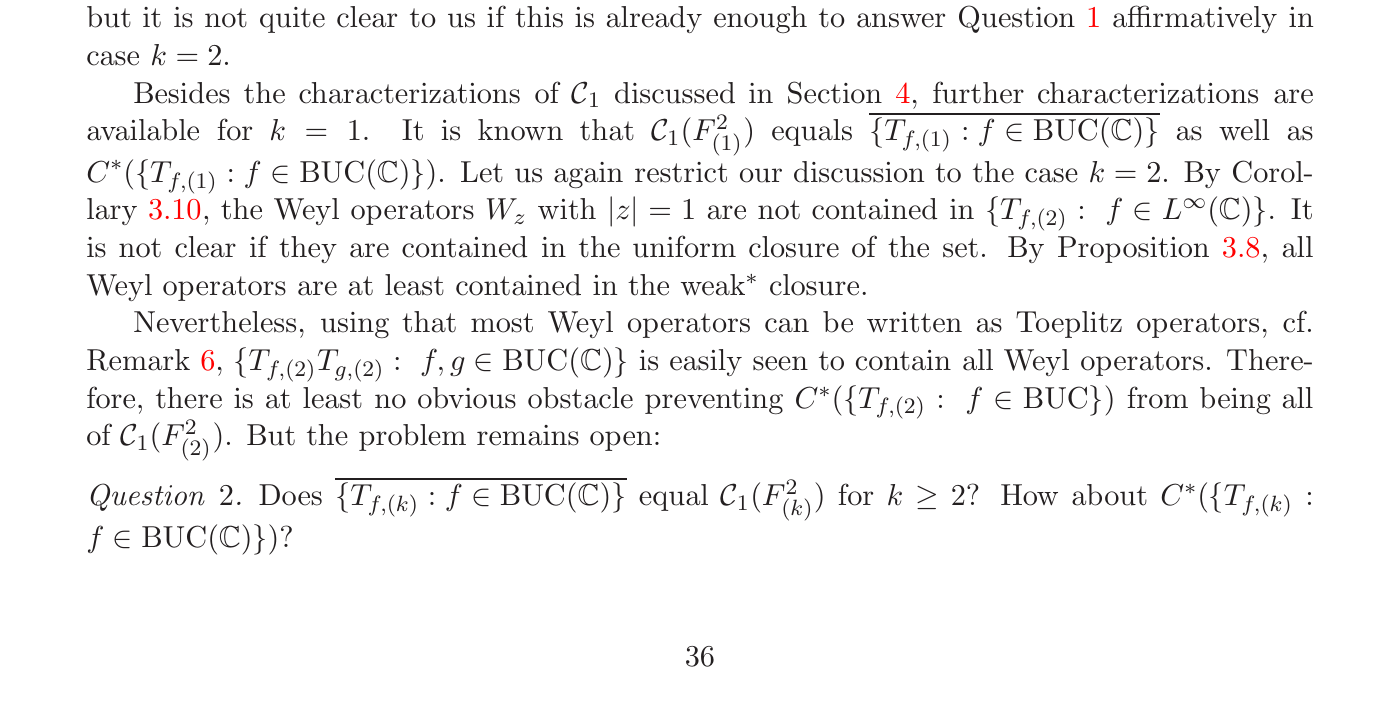
\includegraphics[width=0.96\textwidth]{source/source_question_page36.png}
\end{center}
\vspace{-0.7em}
\noindent\emph{Source evidence: arXiv:2308.11292, PDF page 36.}

\section*{Answer}

Put
\[
 \cT_k=\overline{\{T_{f,(k)}:f\in\BUC(\C)\}}^{\|\cdot\|},
 \qquad
 \cA_k=C^*\{T_{f,(k)}:f\in\BUC(\C)\}.
\]

\begin{theorem}\label{thm:main}
For every \(k\geq2\),
\[
 \cT_k\subsetneq\cC_1(F^2_{(k)})
 \qquad\text{and}\qquad
 \cA_k=\cC_1(F^2_{(k)}).
\]
More precisely, if
\[
 Z_k=\{\rho\in\C:L^0_{k-1}(|\rho|^2)=0\},
\]
then, for each \(\rho\in Z_k\),
\[
 \dist\!\left(W_{-\rho},
       \{T_{f,(k)}:f\in L^\infty(\C)\}\right)=1.
\]
\end{theorem}

\paragraph{Proof intuition.}
Toeplitz quantization at level \(k\) is a Fourier multiplier whose multiplier is a Gaussian times \(L^0_{k-1}\). It erases exactly the finitely many frequency circles \(Z_k\). A contractive Fourier--Følner average isolates a single erased Weyl frequency, proving that it cannot even be approximated in norm by individual Toeplitz operators. Multiplication changes the picture: any Weyl operator is a product of two Toeplitz Weyl operators at non-erased frequencies. Those generated Weyl operators can shift a compact operator spectrum away from \(Z_k\); there the level-\(k\) multiplier is locally invertible. Compact-spectrum approximation then recovers every shift-continuous operator.

\section*{Fourier--Weyl setup}

Write
\[
 S_k=k_{0,(k)}\otimes k_{0,(k)},\qquad Q_k(f)=S_k*f.
\]
Up to the common harmless scalar used in the source, \(Q_k(f)=T_{f,(k)}\). The source proves \cite[Proposition 3.2 and (3.7)]{FH}
\begin{equation}\label{eq:mult}
 m_k(\xi):=\cF_W(S_k)(\xi)
 =e^{-|\xi|^2/2}L^0_{k-1}(|\xi|^2).
\end{equation}
Thus \(Z_k=m_k^{-1}(0)\) is a finite nonempty union of concentric circles for \(k\geq2\). For
\[
 \gamma_\xi(w)=e^{i\sigma(\xi,w)},
\]
the convolution theorem gives \cite[Remark 6]{FH}
\begin{equation}\label{eq:char}
 Q_k(\gamma_\xi)=c_k(\xi)W_{-\xi},
 \qquad c_k(\xi)\neq0\ \Longleftrightarrow\ \xi\notin Z_k.
\end{equation}
Both \(f\mapsto Q_k(f)\) and the shift action are weak-\(^*\) continuous, and
\begin{equation}\label{eq:cov}
 \alpha_z(Q_k(f))=Q_k(\alpha_z f),
 \qquad(\alpha_z f)(w)=f(w-z).
\end{equation}

\section*{The sharp obstruction to linear norm density}

Fix \(\rho\in Z_k\). For \(R>0\), define
\[
 P_R(A)=\frac1{|B_R|}\int_{B_R}
 e^{i\sigma(\rho,z)}\alpha_z(A)\,dz .
\]
For \(A\in\cC_1\) this is a Bochner integral, and \(\|P_R(A)\|\leq\|A\|\).
The Weyl relations give
\[
 \alpha_z(W_{-\rho})=e^{-i\sigma(\rho,z)}W_{-\rho},
 \qquad P_R(W_{-\rho})=W_{-\rho}.
\]

For \(f\in L^\infty(\C)\), covariance \eqref{eq:cov} gives
\[
 P_R(Q_k(f))=Q_k(g_R),\qquad
 g_R=\frac1{|B_R|}\int_{B_R}
 e^{i\sigma(\rho,z)}\alpha_z(f)\,dz .
\]
The net \((g_R)\) is bounded in \(L^\infty\). If a subnet converges weak-\(^*\) to \(g\), the Følner property
\[
 \frac{|(B_R+y)\mathbin{\triangle}B_R|}{|B_R|}\longrightarrow0
\]
implies
\[
 \alpha_y(g)=e^{-i\sigma(\rho,y)}g\qquad(y\in\C).
\]
Consequently \(g\overline{\gamma_\rho}\) is translation invariant, hence a.e.\ constant, so \(g=c\gamma_\rho\). But \(\rho\in Z_k\), and therefore \eqref{eq:char} gives \(Q_k(g)=0\). Weak-\(^*\) continuity of \(Q_k\) now shows that
\[
 P_R(Q_k(f))\longrightarrow0
 \quad\text{ultraweakly}.
\]
Contractivity of \(P_R\) and lower semicontinuity of the operator norm under ultraweak convergence yield
\begin{align*}
 \|W_{-\rho}-Q_k(f)\|
 &\geq \|P_R(W_{-\rho}-Q_k(f))\|\\
 &=\|W_{-\rho}-P_R(Q_k(f))\|,\\
 \|W_{-\rho}-Q_k(f)\|
 &\geq\liminf_{R\to\infty}
 \|W_{-\rho}-P_R(Q_k(f))\|
 \geq\|W_{-\rho}\|=1.
\end{align*}
The choice \(f=0\) gives the reverse inequality. The distance is exactly \(1\), and the first assertion of Theorem~\ref{thm:main} follows.

\section*{Why multiplication recovers all of \(\mathcal C_1\)}

\begin{lemma}\label{lem:weyl}
Every Weyl operator belongs to \(\cA_k\).
\end{lemma}

\begin{proof}
Equation \eqref{eq:char} gives \(W_{-\xi}\in\cA_k\) whenever \(\xi\notin Z_k\). Given arbitrary \(\eta\), choose
\[
 a\notin Z_k\cup(\eta-Z_k).
\]
Then \(a,\eta-a\notin Z_k\). Hence \(W_{-a}\) and \(W_{-(\eta-a)}\) belong to \(\cA_k\), while their product is a unimodular scalar times \(W_{-\eta}\).
\end{proof}

We use three standard facts about the Arveson spectrum
\(\operatorname{sp}_\alpha(A)\) of the norm-continuous action \(\alpha\):
\begin{equation}\label{eq:specfacts}
\begin{split}
 \operatorname{sp}_\alpha(h*A)&\subseteq\operatorname{supp}\widehat h,\\
 \widehat\psi=1\text{ near }\operatorname{sp}_\alpha(A)
 &\Longrightarrow\psi*A=A,\\
 \operatorname{sp}_\alpha(W_\eta A)
 &=\operatorname{sp}_\alpha(A)+\varepsilon\eta
\end{split}
\end{equation}
for the fixed convention-dependent sign \(\varepsilon\in\{1,-1\}\). These follow directly by taking the Fourier transform of the orbit \(z\mapsto\alpha_z(A)\).

\begin{lemma}\label{lem:local}
If \(B\in\cC_1\) has compact Arveson spectrum \(K\) with \(K\cap Z_k=\varnothing\), then \(B\in\cT_k\).
\end{lemma}

\begin{proof}
Transport the irreducible Weyl representation on \(F^2_{(k)}\) unitarily to the analytic Fock representation. Under this identification \(Q_k\) has multiplier \(m_k\), whereas analytic Toeplitz quantization \(Q_1\) has the nowhere-zero multiplier
\[
 m_1(\xi)=e^{-|\xi|^2/2}.
\]
The analytic correspondence theorem says
\begin{equation}\label{eq:analytic}
 \cC_1=\overline{Q_1(\BUC(\C))}^{\|\cdot\|}
\end{equation}
\cite[Theorem 3.1]{F}; the source also recalls this fact immediately before Question 2.

Choose \(\psi\in\mathcal S(\C)\) such that
\[
 \widehat\psi=1\text{ near }K,\qquad
 \operatorname{supp}\widehat\psi\cap Z_k=\varnothing.
\]
Then \(\psi*B=B\) by \eqref{eq:specfacts}. From \eqref{eq:analytic}, choose \(b_j\in\BUC\) with \(Q_1(b_j)\to B\). Hence
\[
 Q_1(\psi*b_j)=\psi*Q_1(b_j)\longrightarrow B.
\]
Define \(\theta\in\mathcal S(\C)\) by
\[
 \widehat\theta(\xi)
 =\frac{m_1(\xi)}{m_k(\xi)}\widehat\psi(\xi).
\]
The quotient is smooth on \(\operatorname{supp}\widehat\psi\), so this is legitimate. Put \(f_j=\theta*b_j\in\BUC\). In tempered Fourier--Weyl distributions,
\[
\begin{aligned}
 \cF_W(Q_k(f_j))
 &=m_k\widehat\theta\,\widehat b_j\\
 &=m_1\widehat\psi\,\widehat b_j
 =\cF_W(Q_1(\psi*b_j)).
\end{aligned}
\]
Injectivity of the tempered Fourier--Weyl transform gives
\[
 Q_k(f_j)=Q_1(\psi*b_j)\longrightarrow B.
\]
Thus \(B\in\cT_k\).
\end{proof}

\begin{proof}[Completion of the proof of Theorem~\ref{thm:main}]
Every \(Q_k(f)\) with \(f\in\BUC\) is shift-continuous, and \(\cC_1\) is a \(C^*\)-algebra; therefore \(\cA_k\subseteq\cC_1\).

Conversely, let \(A\in\cC_1\). Choose an \(L^1\) approximate identity \((h_n)\) whose symplectic Fourier transforms have compact support. Norm continuity of the orbit gives
\[
 A_n=h_n*A\longrightarrow A,
 \qquad
 K_n:=\operatorname{sp}_\alpha(A_n)
 \subseteq\operatorname{supp}\widehat h_n.
\]
The set \(Z_k\) is bounded. Choose \(\eta_n\) and the sign in \eqref{eq:specfacts} so that
\[
 (K_n+\varepsilon\eta_n)\cap Z_k=\varnothing.
\]
Then \(B_n=W_{\eta_n}A_n\) has compact spectrum disjoint from \(Z_k\). Lemma~\ref{lem:local} gives \(B_n\in\cT_k\subseteq\cA_k\), while Lemma~\ref{lem:weyl} gives \(W_{\eta_n}\in\cA_k\). Hence
\[
 A_n=W_{\eta_n}^*B_n\in\cA_k.
\]
Taking the norm limit proves \(A\in\cA_k\), so \(\cA_k=\cC_1\).
\end{proof}

\section*{Scope and provenance}

This settles every clause of the source's Question 2 for every \(k\geq2\). It does not claim an answer to the separate compactness-modulo-Berezin-kernel Question 1. Exact arXiv-id, title, quotation, author, and core-keyword searches through 13 August 2026, together with a direct-citation scan of the published source, found no later arXiv theorem settling Question 2. The proof above is a new result from this run. Its external inputs are the source's explicit multiplier, character, covariance, and tempered Fourier--Weyl identities, plus the analytic correspondence theorem \eqref{eq:analytic}.

\begin{thebibliography}{9}
\bibitem{FH}
R.~Fulsche and R.~Hagger,
\emph{Quantum harmonic analysis for polyanalytic Fock spaces},
arXiv:2308.11292 (2023; revised 2024).
See Proposition 3.2, Remark 6, and Question 2 on PDF page 36.

\bibitem{F}
R.~Fulsche,
\emph{Correspondence theory on \(p\)-Fock spaces with applications to Toeplitz algebras},
arXiv:1911.12668; J. Funct. Anal. 279 (2020), 108661.
\end{thebibliography}

\end{document}
